\documentclass{article}
\usepackage{amsmath}
\usepackage{amssymb}
\usepackage{graphicx}
\usepackage{hyperref}
\usepackage[version=4]{mhchem}

\title{Example 7}
\date{}

\begin{document}
\maketitle

In \(\triangle A B C, A B>A C\). \(M\) is the midpoint of \(B C . A D\) is the angle bisector of \(\angle A\). \(C E \perp A D\) at \(E\). Prove:

\[
M E=\frac{1}{2}(A B-A C) .
\]

\begin{center}
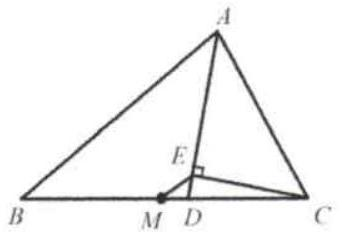
\includegraphics[width=\textwidth]{images/problem_image_1.jpg}
\end{center}


Solution:
Extend \(C E\) to meet \(A B\) at \(F\).\\
Since \(A E \perp C F\) and \(A E\) is the angle bisector of \(\angle A, A E\) is the perpendicular bisector of \(C F\). Thus \(F E=E C, A C=A F\), and \(E\) is the midpoint of \(C F\).\\
Therefore, \(M E\) is the midline of \(\triangle C B F\), and\\
\centering
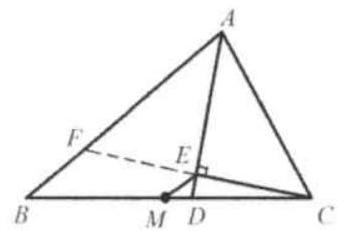
\includegraphics[width=\textwidth]{images/reasoning_image_1.jpg}\\
\(M E=\frac{1}{2} B F=\frac{1}{2}(A B-A F)=\frac{1}{2}(A B-A C)\).


\end{document}
